\documentclass[10pt]{article}
\usepackage[ngerman]{babel}
\usepackage[utf8]{inputenc}
\usepackage[T1]{fontenc}
\usepackage{amsmath}
\usepackage{amsfonts}
\usepackage{amssymb}
\usepackage[version=4]{mhchem}
\usepackage{stmaryrd}
\usepackage{graphicx}
\usepackage[export]{adjustbox}
\graphicspath{ {./images/} }
\usepackage{bbold}

%New command to display footnote whose markers will always be hidden
\let\svthefootnote\thefootnote
\newcommand\blfootnotetext[1]{%
  \let\thefootnote\relax\footnote{#1}%
  \addtocounter{footnote}{-1}%
  \let\thefootnote\svthefootnote%
}

%Overriding the \footnotetext command to hide the marker if its value is `0`
\let\svfootnotetext\footnotetext
\renewcommand\footnotetext[2][?]{%
  \if\relax#1\relax%
    \ifnum\value{footnote}=0\blfootnotetext{#2}\else\svfootnotetext{#2}\fi%
  \else%
    \if?#1\ifnum\value{footnote}=0\blfootnotetext{#2}\else\svfootnotetext{#2}\fi%
    \else\svfootnotetext[#1]{#2}\fi%
  \fi
}

\begin{document}
\section*{Beschreibende Statistik}
\section*{Absolute Häufigkeiten}
$$
H=\sum_{1}^{n} h_{i}
$$

\section*{Relative Häufigkeiten}
$$
F=\sum_{1}^{m} f_{i}, \quad F(x)=\frac{H(x)}{n}
$$

\section*{Kennwerte (Lagemasse)}
\begin{itemize}
  \item Quantil
\end{itemize}

$$
i=\lceil n \cdot q\rceil, Q=x_{i}=x_{\lceil n \cdot q\rceil}
$$

\begin{itemize}
  \item Interquartilsabstand
\end{itemize}

$$
I Q R=Q_{3}-Q_{1}
$$

\begin{itemize}
  \item Modus\\
$x_{\text {mod }}=$ Häufigste Wert
\end{itemize}

\begin{center}
\begin{tabular}{|l|l|}
\hline
Arithmetisches Mittel & Median \\
$\bar{x}=\frac{1}{n} \sum_{i=1}^{n} x_{i}=\sum_{i=1}^{m} a_{i} \cdot f_{i}$ & $\left\{\begin{array}{c}x_{\left[\frac{n+1}{2}\right]} \quad n \text { ungerade } \\ 0.5 \cdot\left(x_{\left[\frac{n}{2}\right]}+x_{\left[\frac{n}{2}+1\right]}\right) \quad n \text { gerade }\end{array}\right.$ \\
\end{tabular}
\end{center}

Stichprobenvarianz $s^{2}$ (Streumasse)

$$
s^{2}=\frac{1}{n} \sum_{i=1}^{n}\left(x_{i}-\bar{x}\right)^{2}=\overline{x^{2}}-\bar{x}^{2}, \quad\left(s_{k o r}\right)^{2}=\frac{1}{n-1} \sum_{i=1}^{n}\left(x_{i}-\bar{x}\right)^{2}
$$

$$
\left(s_{k o r}\right)^{2}=\frac{n}{n-1} \cdot s^{2}
$$

Standardabweichung $s$ (Streumasse)

$$
s=\sqrt{\frac{1}{n} \sum_{i=1}^{n}\left(x_{i}-\bar{x}\right)^{2}}=\sqrt{\overline{x^{2}}-\bar{x}^{2}}, \quad s_{k o r}=\sqrt{\frac{1}{n-1} \sum_{i=1}^{n}\left(x_{i}-\bar{x}\right)^{2}}
$$

\section*{Begriffe}
\begin{itemize}
  \item $\Omega=$ Grundgesamtheit
  \item $n=$ Anzahl Objekte
  \item $X=$ Stichprobenwerte
  \item $a=$ Ausprägungen
  \item $h=$ Absolute Häufigkeit
  \item $f=$ Relative Häufigkeit
  \item $H=$ Kumulative Absolute Häufigkeit
  \item $F=$ Kumulative Relative Häufigkeit
\end{itemize}

\section*{Boxplot}
\begin{itemize}
  \item $Q_{1}, Q_{2}=x_{\text {med }}, Q_{3}$
  \item $I Q R=Q_{3}-Q_{1}$
  \item Untere Antenne $x_{u}: u=\min \left[Q_{1}-1.5 \cdot I Q R, Q_{1}\right]$
  \item Obere Antenne $x_{0}: \quad o=\max \left[Q_{3}+1.5 \cdot I Q R, Q_{3}\right]$
  \item Ausreisser: $\quad x_{i}<x_{u} \vee x_{i}>x_{0}$\\
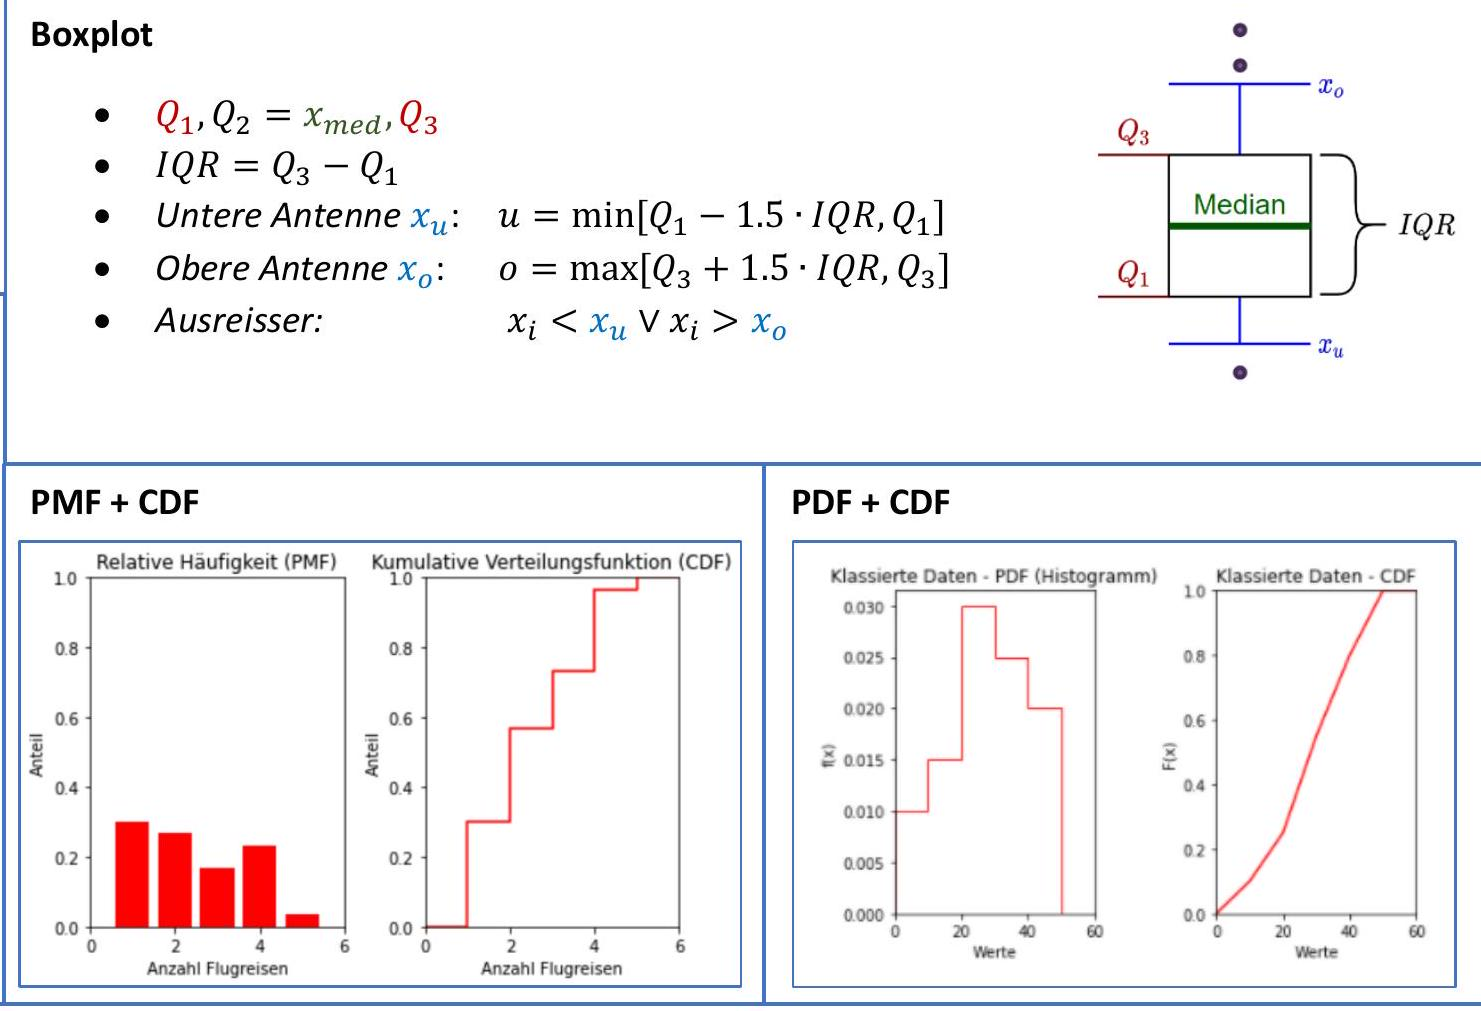
\includegraphics[max width=\textwidth, center]{2024_12_29_e932069dd64ad17e4875g-01(1)}
\end{itemize}

\section*{PDF + CDF}
\begin{center}
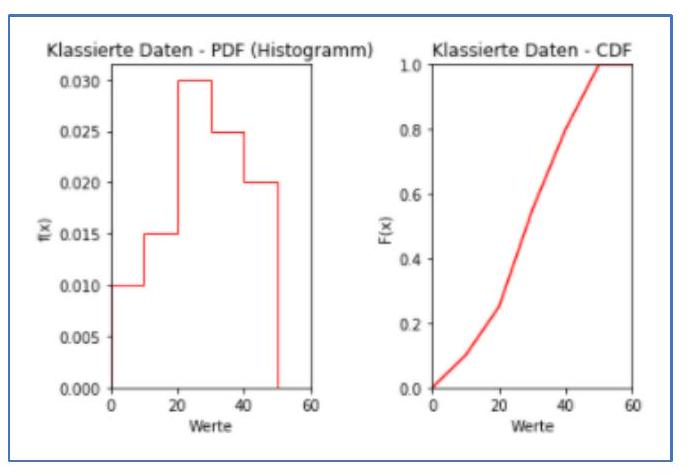
\includegraphics[max width=\textwidth]{2024_12_29_e932069dd64ad17e4875g-01}
\end{center}

\section*{Nicht klassierte Daten (PMF und CDF)}
Die absolute Häufigkeit kann als Funktion $h: \mathbb{R} \rightarrow \mathbb{R}$ bezeichnet werden.

$$
h_{i}
$$

Die relative Häufigkeit kann als Funktion $f: \mathbb{R} \rightarrow \mathbb{R}$ bezeichnet werden.

$$
f_{i}=\frac{h_{i}}{n}
$$

\section*{Klassenbildung (Faustregeln)}
\begin{itemize}
  \item Die Klassen sollten gleich breit gewählt werden
  \item Die Anzahl der Klassen sollte zwischen 5 und 20 liegen, jedoch $\sqrt{n}$ nicht überschreiben.\\
Beispiel:
\end{itemize}

\begin{center}
\begin{tabular}{|c|c|c|c|c|c|}
\hline
$\boldsymbol{a}_{\boldsymbol{i}}$ & $\mathbf{3 9 7}$ & $\mathbf{3 9 8}$ & $\mathbf{3 9 9}$ & $\mathbf{4 0 0}$ & Total \\
\hline
$\boldsymbol{h}_{\boldsymbol{i}}$ & 1 & 3 & 7 & 5 & 16 \\
\hline
$\boldsymbol{f}_{\boldsymbol{i}}$ & $\frac{1}{16}$ & $\frac{3}{16}$ & $\frac{7}{16}$ & $\frac{5}{16}$ & 1 \\
\hline
$\boldsymbol{H}_{\boldsymbol{i}}$ & 1 & 4 & 11 & 16 &  \\
\hline
$\boldsymbol{F}_{\boldsymbol{i}}$ & $\frac{1}{16}$ & $\frac{4}{16}$ & $\frac{11}{16}$ & $\frac{16}{16}$ &  \\
\hline
\end{tabular}
\end{center}

\begin{center}
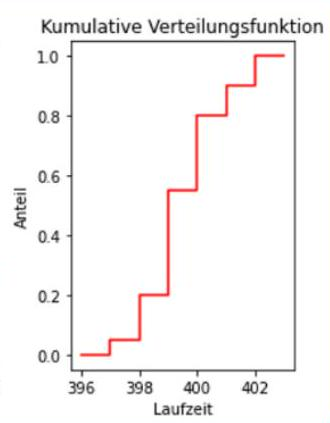
\includegraphics[max width=\textwidth]{2024_12_29_e932069dd64ad17e4875g-02}
\end{center}

\section*{Klassierte Daten (PDF und CDF)}
Die absolute Häufigkeitsdichtefunktion erhält man, indem der Wert der absoluten Häufigkeit $h_{i}$, durch die Klassenbreite (Säulenbreite) $d_{i}$ geteilt wird.

$$
h(x)=\frac{h_{i}}{d_{i}}
$$

Die relative Häufigkeitsdichtefunktion (PDF) $f: \mathbb{R} \rightarrow[0,1]$ erhält man aus der absoluten Häufigkeitsdichtefunktion, indem man den Wert durch die Stichprobengrösse $n$ teilt.

$$
P D F=f(x)=\frac{h(x)}{n}
$$

Beispiel:

\begin{center}
\begin{tabular}{|c|c|c|c|c|c|}
\hline
Klassen & $\mathbf{1 0 0 - 2 0 0}$ & $\mathbf{2 0 0 - 5 0 0}$ & $\mathbf{5 0 0 - \mathbf { 8 0 0 }}$ & $\mathbf{8 0 0 - \mathbf { 1 0 0 0 }}$ & Total \\
\hline
$\boldsymbol{h}_{\boldsymbol{i}}$ & 35 & 182 & 317 & 84 & 618 \\
\hline
$\boldsymbol{f}_{\boldsymbol{i}}$ & $\frac{35}{618}$ & $\frac{182}{618}$ & $\frac{317}{618}$ & $\frac{84}{618}$ & Area $=1$ \\
\hline
$\boldsymbol{d}_{\boldsymbol{i}}$ & 100 & 300 & 300 & 200 &  \\
\hline
$\boldsymbol{h}(\boldsymbol{x})$ & $\frac{35}{100}$ & $\frac{182}{300}$ & $\frac{317}{300}$ & $\frac{84}{200}$ &  \\
\hline
$\boldsymbol{f}(\boldsymbol{x})$ & $\frac{35}{100 \cdot 618}$ & $\frac{182}{300 \cdot 618}$ & $\frac{317}{300 \cdot 618}$ & $\frac{84}{200 \cdot 618}$ &  \\
\hline
\end{tabular}
\end{center}

\begin{center}
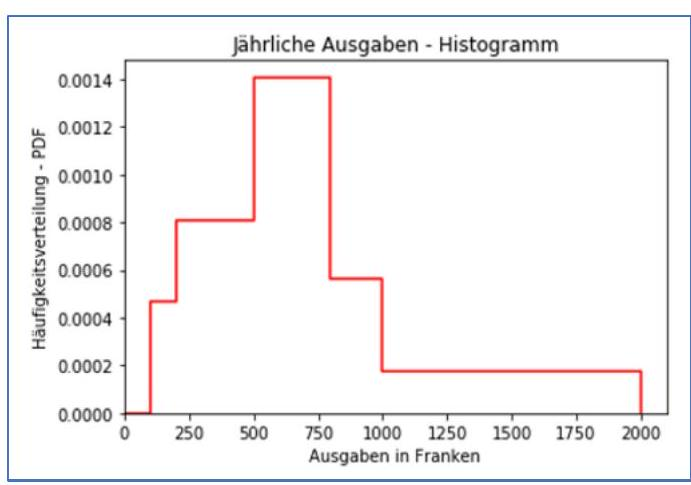
\includegraphics[max width=\textwidth]{2024_12_29_e932069dd64ad17e4875g-02(1)}
\end{center}

\section*{Deskriptive Statistik}
Varianz $s_{x}^{2}, s_{y}^{2}$

$$
\left(s_{x}\right)^{2}=\overline{x^{2}}-\bar{x}^{2}, \quad\left(s_{y}\right)^{2}=\overline{y^{2}}-\bar{y}^{2}
$$

Kovarianz $s_{x y}$

$$
s_{x y}=\frac{1}{n} \sum_{i=1}^{n}\left(x_{i}-\bar{x}\right)\left(y_{i}-\bar{y}\right), \quad s_{x y}=\overline{x y}-\bar{x} \cdot \bar{y}
$$

$$
\begin{aligned}
& \text { Abkürzungen } \\
& \qquad \begin{array}{c}
\bar{x}=\frac{1}{n} \sum_{i=1}^{n} x_{i} \\
\bar{y}=\frac{1}{n} \sum_{i=1}^{n} y_{i} \\
\overline{x y}=\frac{1}{n} \sum_{i=1}^{n} x_{i} \cdot y_{i}
\end{array}
\end{aligned}
$$

Varianz (Ränge) $\left(s_{r g(x)}\right)^{2},\left(s_{r g(y)}\right)^{2}$

$$
\left(s_{r g(x)}\right)^{2}=\overline{r g(x)^{2}}-(\overline{r g(x)})^{2}, \quad\left(s_{r g(y)}\right)^{2}=\overline{r g(y)^{2}}-(\overline{r g(y)})^{2}
$$

Kovarianz (Ränge) $s_{r g(x y)}$

$$
s_{r g(x y)}=\overline{r g(x y)}-\overline{r g(x)} \cdot \overline{r g(y)}=\overline{r g(x y)}-\frac{(n+1)^{2}}{4}
$$

Der Korrelationskoeffizient (Pearson) $r_{x y}$

$$
r_{x y}=\frac{s_{x y}}{s_{x} \cdot s_{y}}=\frac{\overline{x y}-\bar{x} \cdot \bar{y}}{\sqrt{\overline{x^{2}}-\bar{x}^{2}} \cdot \sqrt{\overline{y^{2}}-\bar{y}^{2}}}
$$

Ist der Korrelationskoeffizient $r_{x y}$

\begin{itemize}
  \item $r_{x y} \approx 1 \rightarrow \quad$ starker positiver linearer Zusammenhang
  \item $\quad r_{x y} \approx-1 \rightarrow$ starker negativer linearer Zusammenhang
  \item $\quad r_{x y} \approx 0 \rightarrow \quad$ Keine lineare Korrelation
\end{itemize}

Bemerkungen\\
Auch wenn zwischen zwei Grössen eine Korrelation besteht, so muss das noch lange nicht einen kausalen Zusammenhang bedeuten. Man spricht von Scheinkorrelation.

\section*{Graphische Darstellung}
\begin{itemize}
  \item Form linear / gekrümmt
  \item Richtung positiver / negativer Zusammenhang
  \item Stärke starke / schwache Streuung
\end{itemize}

Korrelationskoeffizient (Spearman) $r_{s p}$

$$
r_{s p}=\frac{s_{r g(x y)}}{s_{r g(x)} \cdot s_{r g(y)}}=\frac{\overline{r g(x y)}-\overline{r g(x)} \cdot \overline{r g(y)}}{\sqrt{\overline{r g(x)^{2}}-(\overline{r g(x)})^{2}} \cdot \sqrt{\overline{r g(y)^{2}}-(\overline{r g(y)})^{2}}}
$$

Vereinfachte Formel, sofern alle Ränge unterschiedlich sind

$$
r_{s p}=1-\frac{6 \cdot \sum_{i=1}^{n} d_{i}^{2}}{n \cdot\left(n^{2}-1\right)}, \quad \text { mit } d_{i}=r g\left(x_{i}\right)-r g\left(y_{i}\right)
$$

\section*{Ränge}
Der Rang $\operatorname{rg}\left(x_{i}\right)$ des Stichprobenwertes $x_{i}$ ist definiert als der Index von $x_{i}$ in der nach der Grösse geordneten Stichprobe.

\begin{center}
\begin{tabular}{|c|c|c|c|c|c|c|}
\hline
$\boldsymbol{i}$ & $\mathbf{1}$ & $\mathbf{2}$ & $\mathbf{3}$ & $\mathbf{4}$ & $\mathbf{5}$ & $\mathbf{6}$ \\
\hline
$\boldsymbol{x}_{\boldsymbol{i}}$ & 23 & 27 & 35 & 35 & 42 & 59 \\
\hline
$\boldsymbol{r}\left(\boldsymbol{x}_{\boldsymbol{i}}\right)$ & 1 & 2 & $\mathbf{3 . 5}$ & $\mathbf{3 . 5}$ & 5 & 6 \\
\hline
\end{tabular}
\end{center}

\section*{Bivariate Daten (Merkmale)}
\begin{itemize}
  \item 2x kategoriell
  \item $1 x$ kategoriell $+1 x$ metrisch
  \item 2x metrisch Kontingenztabelle + Mosaikplot\\
Boxplot oder Striptchart\\
Streudiagramm
\end{itemize}

\section*{Kombinatorik}
\section*{Fakultät}
$$
n!=1 \cdot 2 \cdot \ldots \cdot n=\prod_{k=1}^{n} k
$$

\section*{Binomialkoeffizient}
Wie viele Möglichkeiten gibt es $k$ Objekte aus einer Gesamtheit von $n$ Objekten auszuwählen.

$$
\binom{n}{k}=\frac{n!}{(n-k)!\cdot k!}
$$

\section*{Systematik}
\begin{itemize}
  \item $k$ Anzahl Stellen
  \item $n$ Anzahl Optionen pro Stelle
\end{itemize}

\begin{center}
\begin{tabular}{|c|c|c|c|}
\hline
\multicolumn{2}{|c|}{Variation (mit Reihenfolge)} & \multicolumn{2}{c|}{Kombination (ohne Reihenfolge)} \\
\hline
Mit Wiederholung & Ohne Wiederholung & Mit Wiederholung & Ohne Wiederholung \\
\hline
$n^{k}$ & $\frac{n!}{(n-k)!}$ & $\binom{n+k-1}{k}$ & $\binom{n}{k}$ \\
\hline
Zahlenschloss & Schwimmwettkampf & Zahnarzt & Lotto \\
\hline
\end{tabular}
\end{center}

\section*{Variation mit Wiederholung (Zahlenschloss)}
Wie viele Möglichkeiten gibt es bei einem Zahlenschloss ( 0 - 9) mit 6 Zahlenkränzen?

$$
\begin{gathered}
n=10, \quad k=6 \\
n^{k}=10^{6}
\end{gathered}
$$

\section*{Kombination mit Wiederholung (Zahnarzt)}
3 Spielzeuge werden aus 5 Töpfen gezogen. Jeder Topf ist mit einer (unterschiedlichen) Art von Spielzeug befüllt.

Wie viele Möglichkeiten hat das Kind?

$$
\begin{gathered}
n=5, \quad k=3 \\
\binom{n+k-1}{k}=\binom{5+3-1}{3}=\binom{7}{3}
\end{gathered}
$$

Variation ohne Wiederholung (Schimmwettkampf)\\
Bei einem Schwimmwettkampf starten 10 Teilnehmer. Wie viele mögliche Platzierungen der ersten drei Plätze (Podest) gibt es?

$$
\begin{gathered}
n=10, \quad k=3 \\
\frac{n!}{(n-k)!}=\frac{10!}{(10-3)!}=\frac{10!}{(7)!}
\end{gathered}
$$

\section*{Kombination ohne Wiederholung (Lotto)}
Wie gross sind die Chancen beim Lotto 6 aus 49 Zahlen richtig zu ziehen?\\
Jede Zahl ist nur einmal vorhanden und die Zahlen werden nicht zurückgelegt. Die Reihenfolge in der gezogen wird spielt keine Rolle.

$$
\begin{gathered}
n=49, \quad k=6 \\
\binom{n}{k}=\binom{49}{6}
\end{gathered}
$$

\section*{Ideen}
\begin{itemize}
  \item Berechnung durch Aufteilung in mehrere Kombinationen
  \item Berechnung über Inverse
  \item Prozente = Wahrscheinlichkeit / Gesamt-Wahrscheinlichkeit
\end{itemize}

\section*{Wahrscheinlichkeit, dass ein Ereignis x-Mal Auftritt}
Beim Rommé spielt man mit 110 Karten: sechs davon sind Joker. Zu Beginn eines Spiels erhält jeder Spieler genau 12 Karten.

In wieviel Prozent aller möglichen Fälle sind darunter genau zwei Joker?

$$
\frac{\binom{6}{2} \cdot\binom{104}{10}}{\binom{110}{12}}
$$

In wieviel Prozent aller möglichen Fälle ist darunter mindestens ein Joker?

$$
1-\frac{\binom{104}{12}}{\binom{110}{12}}
$$

Von 100 Glühbirnen sind genau drei defekt. Es werden nun 6 Glühbirnen zufällig ausgewählt.

Wie viele Möglichkeiten gibt es, wenn sich mindestens eine defekte Glühbirne in der Auswahl befinden soll?

$$
\binom{100}{6}-\binom{97}{6}=203^{\prime} 880^{\prime} 032
$$

Mit wie viel Prozent Chancen ist bei einer Auswahl von 6 Glühbirnen keine defekt?

$$
\frac{\binom{97}{6}}{\binom{100}{6}}
$$

Ergebnisraum $\Omega$ : Menge aller möglichen Ergebnisse des Zufallsexperiments. Zähldichte $\rho: \Omega \rightarrow[0,1]$, die jedem Ereignis seine Wahrscheinlichkeit zuordnet.

Für jedes Ereignis aus $\Omega$ gleichwahrschenlich ist, wird $(\Omega, P)$ Laplace-Raum genannt.

$$
P(M)=\frac{|M|}{|\Omega|}
$$

Zwei Ereignisse $A$ und $B$ heissen stochastisch unabhängig, falls

$$
P(A \cap B)=P(A) \cdot P(B)
$$

Zwei Zufallsvariablen $X: \Omega \rightarrow \mathbb{R}$ und $Y: \Omega \rightarrow \mathbb{R}$ heissen stochastisch abhängig, falls

$$
P(X=x, Y=y)=P(X=x) \cdot P(Y=y), \quad f \text { ür alle } x, y \in \mathbb{R}
$$

Für stochastisch unabhängige Zufallsvariablen $X$ und $Y$ gilt

$$
E(X \cdot Y)=E(X) \cdot E(Y), \quad V(X+Y)=V(X)+V(Y)
$$

Wahrscheinlichkeit eines Ereignisses $B$ mit Vorbedingung $A$

$$
P(B \mid A)=\frac{P(B \cap A)}{P(A)}
$$

\section*{Multiplikationssatz}
$$
P(A \cap B)=P(A) \cdot P(B \mid A)=P(B) \cdot P(A \mid B)
$$

Satz von der Totalen Wahrscheinlichkeit

$$
P(B)=P(A) \cdot P(B \mid A)+P(\bar{A}) \cdot P(B \mid \bar{A})
$$

Satz von Bayes

$$
P(A \mid B)=\frac{P(A) \cdot P(B \mid A)}{P(B)}
$$

\begin{center}
\begin{tabular}{|c|c|c|c|}
\hline
 & $A$ & $\bar{A}$ & $\Sigma$ \\
\hline
$B$ & $P(A \cap B)$ & $P(\bar{A} \cap B)$ & $P(B)$ \\
\hline
$\bar{B}$ & $P(A \cap \bar{B})$ & $P(\bar{A} \cap \bar{B})$ & $P(\bar{B})$ \\
\hline
$\Sigma$ & $P(A)$ & $P(\bar{A})$ & $P(\Omega)$ \\
\hline
\end{tabular}
\end{center}

\section*{Spezielle Verteilung (Summary)}
Diskret

$$
\begin{gathered}
E(X)=\sum_{x \in \mathbb{R}} f(x) \cdot x \\
V(X)=\sum_{x \in \mathbb{R}} f(x) \cdot(x-E(X))^{2}
\end{gathered}
$$

Stetig

$$
\begin{gathered}
E(X)=\int_{-\infty}^{\infty} f(x) \cdot x d x \\
V(X)=\int_{-\infty}^{\infty} f(x) \cdot(x-E(X))^{2}
\end{gathered}
$$

\section*{Spezielle Verteilungen}
\section*{Bernoulliverteilung (Einmaliges zurücklegen)}
Bernoulli-Experimente sind Zufallsexperimente mit nur zwei möglichen Ergebnissen. Wir bezeichnen diese Ergebnisse mit 1 und 0.

$$
P(X=1)=p, \quad P(X=0)=1-p=q
$$

\begin{enumerate}
  \item $E(X)=E\left(X^{2}\right)=p$
  \item $V(X)=p \cdot(1-p)$
\end{enumerate}

Eine Hypergeometrische Verteilung kann durch eine Binomialverteilung angenähert werden, wenn $n \leq \frac{N}{20}$

$$
H(N, M, N) \approx B\left(n, \frac{M}{N}\right)
$$

\section*{Approximation durch die Normalverteilung}
\begin{itemize}
  \item Binomialverteilung: $\quad \mu=n p, \sigma^{2}=n p q$
  \item Poissonverteilung: $\quad \mu=\lambda, \sigma^{2}=\lambda$
\end{itemize}

$$
P(a \leq X \leq b)=\sum_{x=a}^{b} P(X=x) \approx \phi_{\mu, \sigma}\left(b+\frac{1}{2}\right)-\phi_{\mu, \sigma}\left(a-\frac{1}{2}\right)
$$

\section*{Faustregel}
Die Approximation (Binomialverteilung) kann verwendet werden, wenn npq $>9$\\
Für grosses $n(n \geq 50)$ und kleiner $p(p \leq 0.1)$ kann Binomial- durch die PoissonVerteilung approximiert werden

$$
B(n, p) \approx \operatorname{Poi}(n \cdot p)
$$

Hypergeometrische Verteilung (Ohne zurücklegen)

\begin{itemize}
  \item $\quad N=$ Objekte gesamthaft
  \item $M=$ Objekte einer bestimmten Sorte
  \item $n=$ Stichprobengrösse
  \item $x=$ Merkmalsträger\\
$P(X=x)=\frac{\binom{M}{x} \cdot\binom{N-M}{n-x}}{\binom{N}{n}}$
\end{itemize}

Schreibweise: $X \sim H(N, M, n)$

\begin{enumerate}
  \item $\mu=E(X)=n \cdot \frac{M}{N}$
  \item $\quad \sigma^{2}=V(X)=n \cdot \frac{M}{n} \cdot\left(1-\frac{M}{N}\right) \cdot \frac{N-n}{N-1}$
  \item $\sigma=S(X)=\sqrt{V(X)}$
\end{enumerate}

Binomialverteilung (Mit zurücklegen)

\begin{itemize}
  \item $n=$ Anzahl Wiederholungen
  \item $\quad p=$ Wahrscheinlichkeit für ein Ergebnis 1
  \item $q=1-p$
  \item 
\end{itemize}

$\square$\\
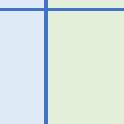
\includegraphics[max width=\textwidth, center]{2024_12_29_e932069dd64ad17e4875g-07}

$$
P(X=x)=\binom{n}{x} \cdot p^{x} \cdot q^{n-x}
$$

Schreibweise: $X \sim B(n ; p)$

\begin{enumerate}
  \item $\mu=E(X)=n p$
  \item $\quad \sigma^{2}=V(X)=n p q$
  \item $\sigma=S(X)=\sqrt{n p q}$
\end{enumerate}

\section*{Poisson Verteilung}
\begin{itemize}
  \item $\lambda=$ Rate
\end{itemize}

$$
P(X=x)=\frac{\lambda^{x}}{x!} \cdot e^{-\lambda}, \quad \lambda>0
$$

Schreibweise $X \sim \operatorname{Poi}(\lambda)$

\begin{enumerate}
  \item $\mu=E(X)=\lambda$
  \item $\sigma^{2}=V(X)=\lambda$
  \item $\sigma=S(X)=\sqrt{\lambda}$
\end{enumerate}

Bei einer stetigen Zufallsvariable $X$ lässt sich die Verteilungsfunktion als Integra einer Funktion $f$ darstellen

$$
F(x)=P(X \leq x)=\int_{-\infty}^{x} f(u) \cdot d u
$$

Liegt eine beliebige Normalverteilung $N(\mu, \sigma)$ vor, muss standardisiert werden. Statt ursprünglichen Zufallsvariablen $X$ betrachtet man die Zufallsvariable

$$
U=\frac{X-\mu}{\sigma}
$$

\section*{Gauss-Verteilung oder Normalverteilung}
Die stetige Zufallsvariable $X$ folgt der Normalverteilung mit den Parametern, $\mu, \sigma \in \mathbb{R}, \sigma>0$, wenn sie folgende Dichtefunktion hat:

$$
\varphi_{\mu, \sigma}(x)=\frac{1}{\sqrt{2 \pi} \cdot \sigma} \cdot e^{-\frac{1}{2}\left(\frac{x-\mu}{\sigma}\right)}
$$

Schreibweise: $X \sim N(\mu ; \sigma)$\\
Ist $\mu=0$ und $\sigma=1$, so spricht man von der Standardnormalverteilung. Ihre Dichtefunktion wird einfach mit $\varphi$ bezeichnet; sie ist gegeben durch

$$
\varphi(x)=\frac{1}{\sqrt{2 \pi}} \cdot e^{-\frac{1}{2} x^{2}}
$$

\section*{Die Verteilungsfunktion der Normalverteilung}
Die kumulative Verteilungsfunktion (CDF) von $\varphi_{\mu, \sigma}(x)$ wird mit $\phi_{\mu, \sigma}(x)$\\
bezeichnet. Sie ist definiert durch

$$
\phi_{\mu, \sigma}(x)=P(X \leq x)=\int_{-\infty}^{x} \varphi_{\mu, \sigma}(t) d t=\frac{1}{\sqrt{2 \pi} \cdot \sigma} \cdot \int_{-\infty}^{x} e^{-\frac{1}{2}\left(\frac{x-\mu}{\sigma}\right)} d t
$$

\section*{Erwartungswert und Varianz der Normalverteilung}
Für eine Zufallsvariable $X \sim N(\mu ; \sigma)$ gilt

$$
E(X)=\mu, \quad V(X)=\sigma^{2}
$$

\section*{Zentraler Grenzwertsatz}
Für eine Folge $X_{1}, X_{2}, \ldots, X_{n}$ von Zufallsvariablen definieren wird die $n$-te Summe $S_{n}$ und das arithmetische Mittel $\bar{X}_{n}$.

Haben alle Zufallsvariablen denselben Erwartungswert $E\left(X_{i}\right)=\mu$ und dieselbe Varianz $V\left(X_{i}\right)=\sigma^{2}$ so folgt

$$
E\left(S_{n}\right)=n \cdot \mu, \quad V\left(S_{n}\right)=n \cdot \sigma^{2}, \quad E\left(\bar{X}_{n}\right)=\mu, \quad V\left(\bar{X}_{n}\right)=\frac{\sigma^{2}}{n}=\frac{1}{n^{2}} \cdot V\left(S_{n}\right)
$$

Sind die Zufallsvariablen alle identisch $N(\mu, \sigma)$ verteilt, so sind die Summe $S_{n}$ und das arithmetische Mittel $\bar{X}_{n}$ wieder normalverteilt mit...

\begin{itemize}
  \item $\quad S_{n}: \quad N(n \cdot \mu, \sqrt{n} \cdot \sigma)$
  \item $\bar{X}_{n}: N\left(\mu, \frac{\sigma}{\sqrt{n}}\right)$
\end{itemize}

Verteilungsfunktion $F_{n}(u)$ der dazugehörigen standardisierten Zufallsvariable

$$
U_{n}=\frac{\left(\left(X_{1}+X_{2}+\cdots+X_{n}\right)-n \mu\right)}{\sqrt{n} \cdot \sigma}=\frac{(\bar{X}-\mu)}{\frac{\sigma}{\sqrt{n}}}
$$

Konvergiert für $n \rightarrow \infty$ gegen die Verteilungsfunktion $\phi(u)$ der Standardnormalverteilung:

$$
\lim _{n \rightarrow \infty} F_{n}(u)=\phi(u)=\frac{1}{\sqrt{2 \pi}} \cdot \int_{-\infty}^{u} e^{-\frac{1}{2} t^{2}} d t
$$

\section*{Methode der kleinsten Quadrate}
\section*{Lineare Regression}
Gegeben sind Datenpunkte ( $x_{i} ; y_{i}$ ) mit $1 \leq i \leq n$. Die Residuen / Fehler $\epsilon_{i}=g\left(x_{i}\right)-y_{i}$ dieser Datenpunkte sind Abstände in $y$-Richtung zwischen $y_{i}$ und der Geraden $g$. Die Ausgleichs- oder Regressiongerade, sei diejenige Gerade für die, die Summe der quadrierten Residuen $\sum_{i=1}^{n} \epsilon_{i}^{2}$ am kleinsten ist.

\section*{Regressionsgerade}
Die Regressionsgerade $g(x)=m x+d$ mit den Parametern $m$ und $d$ ist die Gerade, für welche die Residualvarianz $s_{\epsilon}^{2}$ minimal ist.

Steigung: $m=\frac{s_{x y}}{s_{x}^{2}}, \quad y$-Achsenabschnitt: $d=\bar{y}-m \bar{x}, \quad s_{\epsilon}^{2}=s_{y}^{2}-\frac{s_{x y}^{2}}{s_{x}^{2}}$

\section*{Bestimmtheitsmass}
Die Totale Varianz setzt sich zusammen aus der Residualvarianz und der Varianz der prognostizierten Werte

\begin{itemize}
  \item $s_{y}^{2} \quad$ Totale Varianz
  \item $s_{\hat{y}}^{2} \quad$ prognostizierte (erklärte) Varianz
  \item $s_{\epsilon}^{2}$ Residualvarianz
\end{itemize}

$$
s_{y}^{2}=s_{\epsilon}^{2}+s_{\hat{y}}^{2}
$$

Das Bestimmheitsmass $R^{2}$ beurteilt die globale Anpassungsgüte einer Regression über den Anteil der prognostizierten Varianz $s_{\hat{y}}^{2}$ an der totalen Varianz $s_{y}^{2}$

$$
R^{2}=\frac{s_{\hat{y}}^{2}}{s_{y}^{2}}
$$

Das Bestimmheitsmass $R^{2}$ entspricht dem Quadrat des Korrelationskoeffizienten

$$
R^{2}=\frac{s_{x y}^{2}}{s_{x}^{2} \cdot s_{y}^{2}}=\left(r_{x y}\right)^{2}
$$

\section*{Residuenquadrate}
\begin{itemize}
  \item $y_{i}$ : beobachtete $y-$ Werte
  \item $\hat{y}_{i}$ : prognostizierte bzw. erklärte y-Werte
  \item $\quad \epsilon$ : Residuen (oder auch Fehler)
\end{itemize}

$$
\sum_{i=1}^{n}(\underbrace{y_{i}-g\left(x_{i}\right)}_{\epsilon_{i}})^{2}=\sum_{i=1}^{n}(\underbrace{y_{i}-\hat{y}_{i}}_{\epsilon_{i}})^{2}
$$

\section*{Kleinste Quadrate (KQM)}
Die Parameter $m$ und $q$ werden mit der Matrix $A$ berechnet

$$
A=\left(\begin{array}{cc}
x_{1} & 1 \\
\vdots & \vdots \\
x_{n} & 1
\end{array}\right), \quad A^{T} \cdot A \cdot\binom{m}{q}=A^{T} \cdot\left(\begin{array}{c}
y_{1} \\
\vdots \\
y_{n}
\end{array}\right)
$$

\section*{Linearisierungsfunktionen}
\begin{center}
\begin{tabular}{|c|c|}
\hline
Ausgangsfunktion & Transformation \\
\hline
$\boldsymbol{y}=\boldsymbol{q} \cdot \boldsymbol{x}^{\boldsymbol{m}}$ & $\log (y)=\log (q)+m \cdot \log (x)$ \\
\hline
$\boldsymbol{y}=\boldsymbol{q} \cdot \boldsymbol{m}^{\boldsymbol{x}}$ & $\log (y)=\log (q)+\log (m) \cdot x$ \\
\hline
$\boldsymbol{y}=\boldsymbol{q} \cdot \boldsymbol{e}^{\boldsymbol{m} \cdot \boldsymbol{x}}$ & $\ln (y)=\ln (q)+m \cdot x$ \\
\hline
$\boldsymbol{y}=\frac{\mathbf{1}}{\boldsymbol{q}+\boldsymbol{m} \cdot \boldsymbol{x}}$ & $V=q+m \cdot x ; V=\frac{1}{y}$ \\
\hline
$\boldsymbol{y}=\boldsymbol{q}+\boldsymbol{m} \cdot \ln (\boldsymbol{x})$ & $y=q+m \cdot U ; u=\ln (x)$ \\
\hline
$\boldsymbol{y}=\frac{\mathbf{1}}{\boldsymbol{q} \cdot \boldsymbol{m}^{\boldsymbol{x}}}$ & $\log \left(\frac{1}{y}\right)=\log (q)+\log (m) \cdot x$ \\
\hline
\end{tabular}
\end{center}

\section*{Schliessende Statistik}
\section*{Erwartungstreue Schätzfunktion}
Eine Schätzfunktion $\Theta$ eines Parameters $\theta$ heisst erwartungstreu, wenn

$$
E(\Theta)=\theta
$$

\section*{Effizienz Schätzfunktion}
Gegeben sind zwei erwartungstreue Schätzfunktionen $\Theta_{1}$ und $\Theta_{2}$ desselben Parameters $\theta$. Man nennt $\Theta_{1}$ effizienter als $\Theta_{2}$, falls

$$
V\left(\Theta_{1}\right)<V\left(\Theta_{2}\right)
$$

\section*{Konsistenz Schätzfunktion}
Eine Schätzfunktion $\Theta$ heisst konsistent, wenn

$$
E(\Theta) \rightarrow \theta \text { und } V(\Theta) \rightarrow 0 \text { für } n \rightarrow \infty
$$

Grundgesamtheit mit Erwartungswert $\mu$, Varianz $\sigma^{2}$ und Zufallsstichprobe $X_{1}, X_{2}, X_{3}$. Die folgende Schätzfunktion ist gegeben.

$$
\Theta_{1}=\frac{1}{3} \cdot\left(2 X_{1}+X_{2}\right)
$$

Ist diese Schätzfunktion erwartungstreu (Parameter: $\mu$ )?

$$
\begin{gathered}
E\left(\Theta_{1}\right)=E\left(\frac{1}{3} \cdot\left(2 X_{1}+X_{2}\right)\right)=\frac{1}{3} \cdot\left(2 E\left(X_{1}\right)+E\left(X_{2}\right)\right) \\
E\left(\Theta_{1}\right)=\frac{1}{3} \cdot(2 \mu+\mu)=\frac{3 \mu}{3}=\mu
\end{gathered}
$$

Da $E\left(\Theta_{1}\right)=\mu$ ist die Funktion erwartungstreu.

\section*{Likelyhood-Funktion}
Wir betrachten eine Zufallsvariable $X$ und ihre Dichte (PDF)

$$
f_{x}(x \mid \theta)
$$

Welche von $x$ und einem oder mehreren Parametern $\theta$ abhängig sind. Für eine Stichprobe vom Umfang $n$ mit $x_{1}, \ldots, x_{n}$ nennen wir die vom Parameter $\theta$ abhängige Funktion ... die Likelyhood-Funktion der Stichprobe.

$$
L(\theta)=f_{x}\left(x_{1} \mid \theta\right) \cdot f_{x}\left(x_{2} \mid \theta\right) \cdot \ldots \cdot f_{x}\left(x_{n} \mid \theta\right)
$$

\section*{Vorgehen - Likelyhood Funktion}
\begin{enumerate}
  \item Likelyhood-Funktion bestimmen
  \item Maximalstelle der Funktion bestimmen
\end{enumerate}

\begin{itemize}
  \item (Partielle) Ableitung $L^{\prime}(\theta)=0$
\end{itemize}

\section*{Erwartungswert (Funktion, Wert)}
$$
\bar{X}=\frac{1}{n} \cdot \sum_{i=1}^{n} X_{i}, \quad \hat{\mu}=\bar{x}=\frac{1}{n} \cdot \sum_{i=1}^{n} x_{i}
$$

Varianz (Funktion, Wert)

$$
S^{2}=\frac{1}{n-1} \cdot \sum_{i=1}^{n}\left(X_{i}-\bar{X}\right)^{2}, \quad \hat{\sigma}^{2}=s^{2}=\frac{1}{n-1} \cdot \sum_{i=1}^{n}\left(x_{i}-\bar{x}\right)^{2}
$$

\footnotetext{Pascal Isliker
}\section*{Vertrauensintervalle}
Wir legen eine grosse Wahrscheinlichkeit $\gamma$ fest (z.B. $\gamma=95 \%$ ). $\gamma$ heisst statistische Sicherheit oder Vertrauensniveau. $\alpha=1-\gamma$ ist die sogenannte Irrtumswahrscheinlichkeit.

Dann bestimmen wir zwei Zufallsvariablen $\Theta_{u}$ und $\Theta_{o}$ so, dass sie den wahren Parameterwert $\Theta$ mit der Wahrscheinlichkeit $\gamma$ einschliessen:

$$
P\left(\Theta_{u} \leq \Theta \leq \Theta_{u}\right)=\gamma
$$

\section*{Spezialfall: Anteilswert $\boldsymbol{p}$ einer Bernoulli-Verteilung (Funktion, Wert)}
$$
\bar{X}=\frac{1}{n} \cdot \sum_{i=1}^{n} X_{i}, \quad \hat{p}=\bar{x}=\frac{1}{n} \cdot \sum_{i=1}^{n} x_{i}
$$

\section*{Intervallschätzung}
Geben Sie das Vertrauensintervall für $\mu$ an ( $\sigma^{2}$ unbekannt). Gegeben sind...

$$
n=10, \quad \bar{x}=102, \quad s^{2}=16, \quad \gamma=0.99
$$

\begin{enumerate}
  \item Verteilungstyp bestimmen
\end{enumerate}

Verteilungstyp mit Param $\mu$ und $\sigma^{2}$ unbekannt $\rightarrow T$-Verteilung\\
2. Verteilung und Quantile berechnen

$$
f=n-1=9, \quad p=\frac{1+\gamma}{2}=0.995, \quad c=t_{(p ; f)}=t_{(0.995 ; 9)}=3.25
$$

\begin{enumerate}
  \setcounter{enumi}{2}
  \item Vertrauensintervall bestimmen
\end{enumerate}

$$
e=c \cdot \frac{S}{\sqrt{n}}=4.111, \quad \Theta_{\mathrm{u}}=\bar{X}-e=97.89, \quad \Theta_{\mathrm{o}}=\bar{X}+e=106.11
$$

\begin{center}
\begin{tabular}{|c|c|c|c|c|c|c|}
\hline
 & Verteilung der Grundgesamtheit & Param & Schätzfunktionen & Standardisierte Zufallsvariable & Verteilung / Quantile & Intervallgrenzen \\
\hline
1 & Normalverteilung (Varianz $\sigma^{2}$ bekannt) & $\mu$ & $\bar{X}$ & $U=\frac{(\bar{X}-\mu)}{\sigma / \sqrt{n}}$ & Standardnormalverteilung \( c=u_{p}, p=\frac{1+\gamma}{2} \) & \( \begin{gathered} e=c \cdot \frac{\sigma}{\sqrt{n}} \\ \Theta_{\mathrm{u}}=\bar{X}-e, \quad \Theta_{\mathrm{o}}=\bar{X}+e \end{gathered} \) \\
\hline
2 & \begin{tabular}{l}
Normalverteilung \\
(Varianz $\sigma^{2}$ unbekannt und $n \leq 30$; \\
sonst Fall 1 mit $s$ als Schätzwert für $\sigma$ ) \\
\end{tabular} & $\mu$ & $\bar{X}, \quad S^{2}$ & \( T=\frac{(\bar{X}-\mu)}{S / \sqrt{n}} \) & t-Verteilung \( c=t_{(p ; f=n-1)}, p=\frac{1+\gamma}{2} \) & \( \begin{gathered} e=c \cdot \frac{S}{\sqrt{n}} \\ \Theta_{\mathrm{u}}=\bar{X}-e, \quad \Theta_{\mathrm{o}}=\bar{X}+e \end{gathered} \) \\
\hline
3 & Normalverteilung & $\sigma^{2}$ & $\bar{X}, \quad S^{2}$ & \( Z=(n-1) \frac{s^{2}}{\sigma^{2}} \) & Chi-Quadrat-Verteilung \( \begin{aligned} & c_{1}=z_{\left(p_{1} ; f=n-1\right)}, p_{1}=\frac{1-\gamma}{2} \\ & c_{2}=z_{\left(p_{2} ; f=n-1\right)}, p_{2}=\frac{1+\gamma}{2} \end{aligned} \) & \( \begin{gathered} e=(n-1) \cdot S^{2} \\ \Theta_{u}=\frac{e}{c_{2}}, \quad \Theta_{o}=\frac{e}{c_{1}} \end{gathered} \) \\
\hline
4 & Bernoulli-Verteilung mit $n \hat{p}(1-p)>9$ & $p$ & \( P\left(X_{i}=1\right)=p \) & \( U=\frac{\bar{X}-p}{\sqrt{p(1-p) / n}} \) & Standardnormalverteilung näherungsweise \( c=u_{q}, q=\frac{1+\gamma}{2} \) & \( \begin{gathered} e=c \cdot \sqrt{\frac{\bar{X} \cdot(1-\bar{X})}{n}} \\ \Theta_{u}=\bar{X}-e, \quad \Theta_{o}=\bar{X}+e \end{gathered} \) \\
\hline
5 & Beliebig mit $n>30$ & $\mu, \sigma^{2}$ & \multicolumn{4}{|l|}{Wie im Fall 1 (gegebenenfalls mit $s$ als Schätzwert für $\sigma$ ) bzw. wie im Fall 3} \\
\hline
\end{tabular}
\end{center}

Pascal Isliker


\end{document}